%%%%%%%%%%%%%%%%%%%%%%%%%%%%%%%%%%%%%%%%%%%%
%%% STAFF MAGIC
%%%%%%%%%%%%%%%%%%%%%%%%%%%%%%%%%%%%%%%%%%%%


\mysection{Staff Magic}{wonder-staff-magic}

A staff can be a cane, club, wand, staff, caduceus, or walking stick; it is a necessary accessory for any Philosopher reaching the heights of their study. It must be made out of a special material: the more powerful the staff, the better the material must be.  If you're making an Iron level staff you might need a branch from an ash tree from the Forbidden Wood.  If you're making a Gold level staff, it might need to be the femur of the Great Wyrm Vermithrax.  Work this out with the Arbiter!

All staffs are 2-handed Fast Brawl weapons that do d6 damage.  They can produce light at will (as a torch); can hit creatures only affected by magic weapons; and can dispel \mylink{Illusion}{wizardry-illusion} with a touch (though this will prompt a \mylink{Wizards' Duel}{philosopher-wizards-duel} if the opposing wizard is present).

If you do not wish anyone else to use this staff, it can be bound with a \mylink{Wizard Sigil}{research-sigil-wizard} created by you. As long as the staff has your Wizard Sigil on it, the staff is just a normal quarterstaff in anyone else's hands (though obviously made of special material!).  You must place the Wizard Sigil at the moment you create the staff.

A Staff is limited to 3 powers, but you can "mix and match" from any group as you wish (so the staff could have 2 Iron powers and 1 Gold power if you wanted). These are just the most common abilities; you're encouraged to work out additional abilities with the Arbiter.

The "Stackable" column in the table indicates if the ability can be bought more than once.  When you see \NUM in a description, this is the number of times you bought the ability.

  \begin{center}
    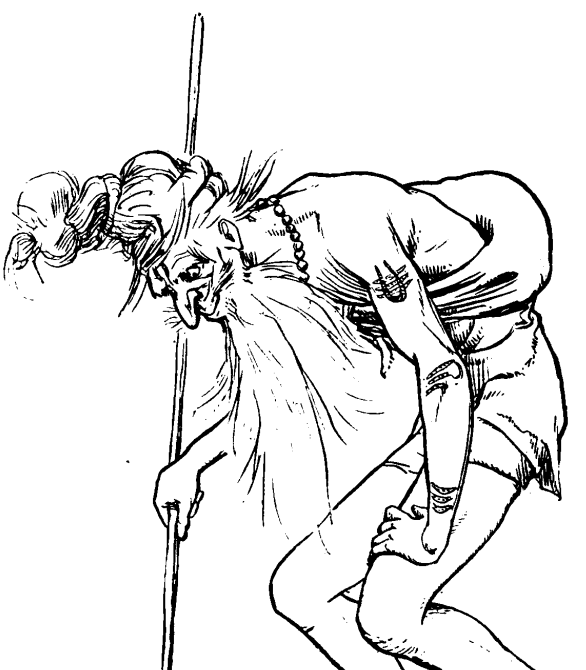
\includegraphics[scale=.5]{StaffMagic}
  \end{center}



\mysubsection{Iron Powers}{staff-magic-iron-powers}

    \example { 
        \COST  500\FE each
    }

  \mytable{X r}{
    \thead{Effect} & \thead{Stackable} \\
  }{
     All Saves +1 & No \\
     Anchor: d8 & No \\
     Blood: 1 & No \\
     Damage +1 & Yes \\    
     Daze & No \\
     Insight: +1 & Yes \\
     Mending & No \\
     Mitigation: Mishap to nothing & No \\
     Safe Casting & Yes \\
     Use your \INT for Fight Rolls\footnote{Instead of \VIG} & No \\
  }

\newpage


\mysubsection{Silver Powers}{staff-magic-silver-powers}
    \example { 
      \COST 1000\AG each
    }

  \mytable{X r}{
    \thead{Effect} & \thead{Stackable} \\
  }{
     All Saves +2 & No \\
     Anchor: d10 & No \\
     Blood: 2 & No \\
     Damage \DCUP & No \\
     Insight: +2 & Yes \\
     Mitigation: Calamity to Mishap & No \\
     Power Casting & Yes \\
     Rend & No \\
     Use your \INT for Fight\ and Guard\footnote{Instead of \DEX}  rolls & No \\
  }


\mysubsection{Gold Powers}{staff-magic-gold-powers}
\example { 
  \COST 2500\AU each
}

  \mytable{X r}{
    \thead{Effect} & \thead{Stackable} \\
  }{
     All Saves +4 & No \\
     Anchor: d12 & No \\
     Blood: 3 & No \\
     Cleave & No \\
     Damage \DCUP & Yes \\
     Insight: +4 & Yes \\
     Mitigation: Ruin to Calamity & No \\
     Natural Casting & Yes \\
     Wisdom & No \\
  }

\cbreak

\myhighlight{Anchor}{staff-magic-anchor}

Changes the die you roll with your \INT when rolling a Torrent,; instead of a d6, use the die listed

\myhighlight{Blood}{staff-magic-blood}

Once per Session, you can tap into the power of the Staff directly and add 1 (Iron), 2 (Silver), or 3 (Gold) Blood Dice to your Pool.

\myhighlight{Insight}{staff-magic-insight}

Up to \NUM times a Session, you can add a +1,+2, or +4 (depending on the level) to any Knowledge roll.  You can only use this ability once per roll i.e.  you cannot use Insight: +2 twice on the same roll to get a +4

\myhighlight{Mending}{staff-magic-mending}

The \TARGET cost of \mylink{Mend}{leechcraft-mend} is 1 as long as the staff is in your possession.


\myhighlight{Mitigation}{staff-magic-mitigation}

Once per Session, Mitigation reduces the effect of a Ruin to a Calamity (Gold); a Calamity to a Mishap (Silver); and eliminates the effect of a Mishap (Iron).

\myhighlight{Natural Casting}{staff-magic-natural casting}

Your Blood Dice are only depleted on a natural 1 (instead of a 1 or 2). 


\myhighlight{Power Casting}{staff-magic-power casting}

You can replace one of your rolled Blood Die with a natural 6 (as if it was rolled) \NUM times per Session  

 

\myhighlight{Safe Casting}{staff-magic-safe casting}

You can replace one of your rolled Blood Die with a natural 1 (as if it was rolled) \NUM times per Session.

\myhighlight{Wisdom}{staff-magic-wisdom}

Whenever you fail a Leechcraft roll, the negative modifier is -1 instead of -2 (the modifiers are still cumulative).

\newpage
